\documentclass{article}

\usepackage{amsmath,amssymb}
\usepackage{mathtools}
\usepackage{hyperref}
\usepackage{amssymb}
\usepackage{graphicx}
\graphicspath{{../logos/}}


\begin{document}

\setlength{\tabcolsep}{5pt}
\begin{center} \begin{tabular}{cccc}
	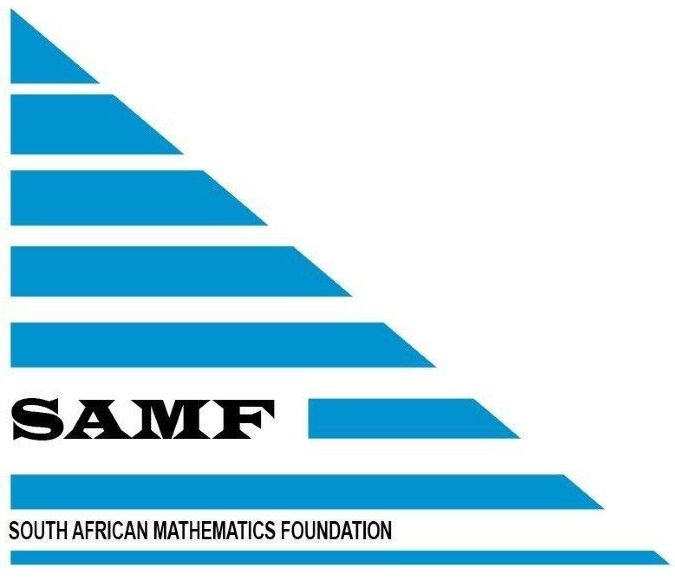
\includegraphics[height=43pt]{SAMF_logo.jpg} &
	
\includegraphics[height=43pt]{SAICA_logo.jpg} &
	
\includegraphics[height=43pt]{OM_Logo_Stacked_Vignette_on_White_RGB.jpg} &
	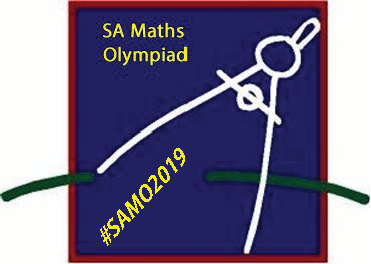
\includegraphics[height=43pt]{SAMO2019.png}
\end{tabular} \end{center}

\bigskip

\begin{center}
\textbf{\Large Senior Monthly Problem Set for when it would have been IMO season :(}
\\ \vspace{1em}
\textbf{\large Due: Saturday, XX XXXX 2020}
\end{center}


\begin{enumerate}

\bigskip
\item[1.] %


\medskip
\item[2.] % AoPS, 2020
For $n,m\in\mathbb{N}$ let $S_{n,m}$ be the set of all increasing integer sequences $x_{1},x_{2},\ldots,x_{nm}$, where $0\leq x_i\leq nm$ and satisfying $n \mid x_{1} + x_{2} + \cdots +x_{nm}$. Prove that exactly half of the elements of $S_{n,m}$ have $x_{nm}=nm$.


\medskip
\item[3.] %


\medskip
\item[4.] % 1997 Romania TST, Day 1, Q3
There are $n$ points in the plane such that no three are collinear and the points do not all lie on the same circle. If $S$ is the set containing these $n$ points, find all functions $f : S \rightarrow \mathbb{R}$ such that all circles that have $m \ge 3$ points, $p_1$, $p_2$, $\dots$, $p_m$, in S satisfy

$$\sum_{i = 1}^{m} f(p_i) = 0.$$



\medskip
\item[5.] %2012 European Girls’ Mathematical Olympiad P8
 A word is a collection of letters. Define a word to be $rhythmical$ if it can be written as the concatenation of $2$ or more identical words (for example, $hehehe$ and $fufufu$ are $rhythmical$, but $hahah$ and $hohohaha$ are not). A word is said to be $melodic$ if after swapping any two differing adjacent letters, the resulting word would be $rhythmical$. Find all $melodic$ words.


\medskip
\item[6.] % 



\medskip
\item[7.] %


\medskip
\item[8.] % Ralph, 2020
Let $f(n)$ be the number of pairs $(p, q)$ such that $p + q = n$ where both $p$ and $q$ are primes. Prove that
$$\sum_{k = 1}^{m} \frac{f(k)}{2^k} < 1$$
for all positive integers $m$.


\end{enumerate}


\vfill
\textbf{\Large Email submission guidelines}
\begin{itemize}
	\item Email your solutions to \href{mailto:samf.training.assignments@gmail.com}{\texttt{samf.training.assignments@gmail.com}}.
	\item In the subject of your email, include your name and the level of the assignment (Beginner, Intermediate or Senior).
	\item Submit each question in a single separate PDF file (with multiple pages if necessary), with your name and the question number written on each page.
	\item If you take photographs of your work, use a document scanner such as Office Lens to convert to PDF.
	\item If you have multiple PDF files for a question, combine them using software such as PDFsam.
\end{itemize}

\end{document}
